%----------------------------------------------%
%                                              %
% Title:  Linux device drivers explained       %
% Author: Giuseppe Calderaro                   %
% Date:   29th October 2009                    %
%                                              %
%----------------------------------------------%

% Latex document class
\documentclass{beamer}
\usepackage{beamerthemeshadow}
\usepackage{listings}
\lstset{language=C}
\setbeamertemplate{navigation symbols}{}
\usetheme{Berkeley}
\beamersetuncovermixins{\opaqueness<1>{25}}{\opaqueness<2->{15}}

% Document start
\begin{document}
\title{Linux Device Drivers explained}
\author{Giuseppe Calderaro}
\institute[http://www.imgtec.com/]{Imagination technologies ltd.}
\date{29th October 2009}

% Slide: 1
\frame{\titlepage}

% Slide: 2
\frame{\frametitle{Table of contents}\tableofcontents}

%% LINUX SYSTEM ARCHITECTURE
% Slide: 3
\section{Linux system architecture}
\subsection{Linux system architecture}
\frame{\frametitle{Linux system architecture}
  \begin{columns}
    \begin{column}{10cm}
      \begin{figure}
        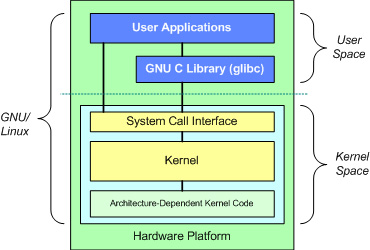
\includegraphics[scale=0.75]{arch1.eps}
        \caption{Linux system architecture}
      \end{figure}
    \end{column}
  \end{columns}
}

% Slide: 4
\subsection{Linux kernel architecture}
\frame{\frametitle{Linux kernel architecture}
  \begin{columns}
    \begin{column}{3cm}
      \begin{figure}
        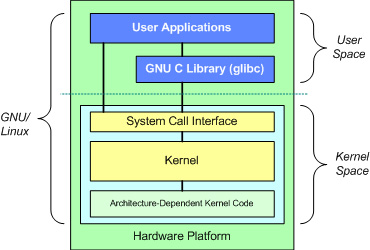
\includegraphics[scale=0.35]{arch1.eps}
        \caption{\tiny{Linux system architecture}}
      \end{figure}
    \end{column}
    \begin{column}{7cm}
      \begin{figure}
        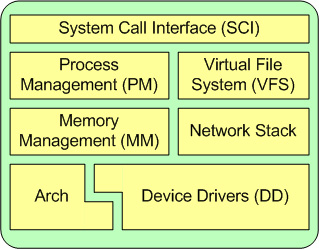
\includegraphics[scale=0.65]{arch2.eps}
        \caption{Linux kernel architecture}
      \end{figure}     
    \end{column}
  \end{columns}
}

%% BUILDING AND RUNNING MODULES
% Slide: 5
\section{Building and running modules}
\subsection{A polite module...}
\frame{\frametitle{A polite module...}
  \makebox{
    \scriptsize{
      \lstinputlisting{example.c}
    }
  }
}

% Slide: 6
\subsection{...and his Makefile}
\frame{\frametitle{...and his Makefile}
  \makebox{
    \scriptsize{
      \lstinputlisting{Module_Makefile}
    }
  }
}

%% DEBUGGING TECHNIQUES
% Slide: 7->9
\section{Debugging techniques}
\subsection{printk}
\frame{\frametitle{printk}
  \begin{itemize}
    \item<1-> printf(''I am printf!'');
    \item<2-> printk(''I am printk!'');
    \item<3-> printf prototype: int printf(const char *format, ...);
    \item<3-> printk prototype: int printk(const char *fmt, ...);
  \end{itemize}
}

% Slide: 10->11
\subsection{Log level values}
\frame{\frametitle{Log level values}
  \begin{itemize}
    \item<1-> \lstinputlisting{kernel_1line.h}
    \item<2-> \lstinputlisting{kernel_2line.h}
  \end{itemize}
}

% Slide: 12
\frame{\frametitle{Log level values}
  \makebox{
    \scriptsize{
      \lstinputlisting{kernel.h}
    }
  }
}

% Slide: 13->15
\subsection{mmm... proc... what's that?!?}
\frame{\frametitle{mmm... proc... what's that?!?}
  \begin{itemize}
  \item<1->{
    [giuseppe@wopr ~]\$ cat /proc/sys/kernel/printk\\
    3\hspace{1.5cm}4\hspace{1.5cm}1\hspace{1.5cm}7
  }
  \item<2-> Current Default Minimum Boottime
  \item<3-> echo 8 > /proc/sys/kernel/printk
  \item<3-> if the value is set to 8, all messages, including debugging ones, are displayed.
  \end{itemize}
}

% Slide: 16
\subsection{Other debugging techniques}
\frame{\frametitle{Other debugging techniques}
  \begin{itemize}
    \item Use the /proc filesystem
    \item Use ioctl method
    \item Debugging by watching (strace, ltrace)
    \item Oops messages (continues...)
    \item gdb vmlinux /proc/kcore
    \item kdb kernel debugger
    \item kgdb kernel debugger (in vanilla)
    \item User mode linux (!?!)
    \item Linux Trace Toolkit
    \item Kernel probes (good good)
    \item ice kernel debugger (waited for 4891AD)
  \end{itemize}
}

% Slide: 17
\subsection{OOOOOOOPS!}
\frame{\frametitle{OOOOOOOPS!}
  \tiny{
    \lstinputlisting{oops.txt}
  }
}

% Slide: 18
\section{Concurrency and Race conditions}
\subsection{Semaphores and mutexes}
\frame{\frametitle{Semaphores and mutexes}
  \scriptsize{
    \lstinputlisting{semaphores.txt}
  }  
}

% Slide: 19
\subsection{Reader/writer Semaphores}
\frame{\frametitle{Reader/writer semaphores}
  \tiny{
    \lstinputlisting{rwsem.txt}
  }    
}

% Slide: 20
\subsection{Completions}
\frame{\frametitle{Comple...}
  A common pattern in kernel programming involves initiating some activity outside of
  the current thread, then waiting for that activity to complete.
  \scriptsize{
    \lstinputlisting{completions1.txt}
  }
}

% Slide: 21
\subsection{Completions}
\frame{\frametitle{...tions}
  \scriptsize{
    \lstinputlisting{completions2.txt}
  }
}

% Slide: 22
\subsection{Spinlocks and...}
\frame{\frametitle{Spinlocks and...}
  \tiny{
    \lstinputlisting{spinlocks.txt}
  }  
}

% Slide: 23
\subsection{...Atomic Context!}
\frame{\frametitle{...Atomic Context!}
  In atomic context (interrupt context, softirq context)\\
  YOU CAN'T:
  \begin{itemize}
    \item Schedule
    \item Sleep
    \item Use semaphores (they could go to sleep)
  \end{itemize}
  and\\
  \begin{center}
    YOU MUST USE SPINLOCKS!\\
  \end{center}
  Otherwise:\\
  \begin{center}
    BUG: scheduling while atomic\\
    kernel panic, not syncing. Aiiie, killing interrupt handler...
  \end{center}
}

% Slide: 24
\subsection{Reader/Writer Spinlocks}
\frame{\frametitle{Reader/Writer Spinlocks}
  \tiny{
    \lstinputlisting{rwspinlocks.txt}
  }
}

% Slide: 25
\subsection{Lock-Free Algorithms}
\frame{\frametitle{Lock-Free Algorithms}
  \begin{itemize}
  \item Circular buffers
  \item Atomic variables
  \item Bit operations
  \item seqlocks (continues...)
  \item Read-Copy update (continues...)
  \end{itemize}
}

% Slide: 26
\subsection{seqlocks}
\frame{\frametitle{seqlocks}
  Read access works by obtaining an (unsigned) integer sequence value on entry into
  the critical section. On exit, that sequence value is compared with the current value;
  if there is a mismatch, the read access must be retried. As a result, reader code has a
  form like the following:

  \scriptsize{
    \lstinputlisting{seqlocks.txt}
  }
}

% Slide: 27
\subsection{Read-Copy-Update}
\frame{\frametitle{Read-Copy-Update}
  \tiny{
    \lstinputlisting{rcu.txt}
  }
}

% Slide: 28
\section{Allocating memory}
\subsection{The real story of kmalloc}
\frame{\frametitle{The real story of kmalloc}
  
}

% Slide: 29
\subsection{Lookaside caches}
\frame{\frametitle{Lookaside caches}
  
}

% Slide: 30
\subsection{vmalloc and friends}
\frame{\frametitle{vmalloc and friends}
  
}

% Slide: 31
\section{Communicating with hardware}
\subsection{I/O Ports and I/O Memory}
\frame{\frametitle{I/O Ports and I/O Memory}
  
}

% Slide: 32
\subsection{Using I/O Memory}
\frame{\frametitle{Using I/O Memory}
  
}

% Slide: 33
\section{Interrupt handling}
\subsection{Installing an interrupt handler}
\frame{\frametitle{Installing an interrupt handler}

}

% Slide: 34
\subsection{Top and bottom halves}
\frame{\frametitle{Top and bottom halves}

}

% Slide: 35
\subsection{Title}
\frame{\frametitle{Title}

}

% Document end
\end{document}
